\documentclass[a4paper,12pt]{report}

\usepackage{graphicx}
\usepackage{pgfplots}
\usepackage{graphicx}

\pgfplotsset{compat=1.18}

\title{Report\\ \textbf {``MTSK-GAME''}}

\author{Pietro Olivi\\
Leonardo Tassinari\\
Lorenzo Dalmonte}
\date{\today}


\begin{document}

\maketitle

\tableofcontents

\chapter{Analysis}
The software commissioned by the professors of the Object-Oriented Pro\-gramming course aims to create an application designed to enhance psycho-motor skills through a gaming experience based on multitasking.\\
The term \textit{Multitasking} refers to the ability of a person or a product to do more than one thing at a time.

\section{Requirements}
\subsection*{Functional}
\begin{itemize}
	\item Upon starting, the software will display a simple minigame.\footnote{A minigame is a potentially-never-ending challenge that requires simple actions from the player in order to keep the game going.}
	\item After a short amount of time a new minigame will appear and so on until all four minigames are shown.
	\item Generally, the difficulty of each minigame shall increase over time.
	\item The player's goal is to survive as long as possible. After failing a minigame the application will display the final result,
	      therefore the software has to keep track of how long the player has lasted in the match in order to calculate the score.
	\item It will be possible to appreciate the improvement on a \textit{Statistics} page that will show the record of all the past runs.
\end{itemize}

\subsection*{Non functional}
\begin{itemize}
	\item The application shall sustain acceptable frame rate (around 60 fps) in all the sections of the gameplay, even on older hardware\footnote{e.g. Intel Core i3 (fourth generation), 4Gb of RAM.}.
	\item It shall be possible to easily develop and swap the minigames among the ones that best fit the training purposes of the user on top of those already provided.
	\item It shall be possible to play in full screen mode.
	\item The window shall be resizable to fit in any kind of screen\footnote{Provided a minimum resolution.}.
\end{itemize}



\section{Domain analysis}

MTSK-Game must exhibit some \textit{minigames}, the ones supplied by us are:
\begin{itemize}
	\item \textit{WhacAMole}: where the goal is to crush all the moles that emerge from the dug holes, before they re-enter them, avoiding detonating bombs that will also pop up from the pipes.
	\item \textit{DodgeATriangle}: in which the player has to slide a \textit{rectangle} up and down in a column switching lanes, aiming to avoid hitting moving \textit{triangles}.
	\item \textit{CatchTheSquare}: where the user should destroy \textit{squares} running over them with a \textit{circle} before their timers runs out. With time, multiple squares will spawn at the same time with an increasing rate.
	\item \textit{FlappyBirdAlike}: where the user needs to control a \textit{cursor} leading it to avoid \textit{obstacles} that will come towards it.
\end{itemize}
For the game to end, and the \textit{score} to appear, it'll be sufficient losing in only one of the currently displayed minigames.


\begin{figure}[ht]
	\centering{}
	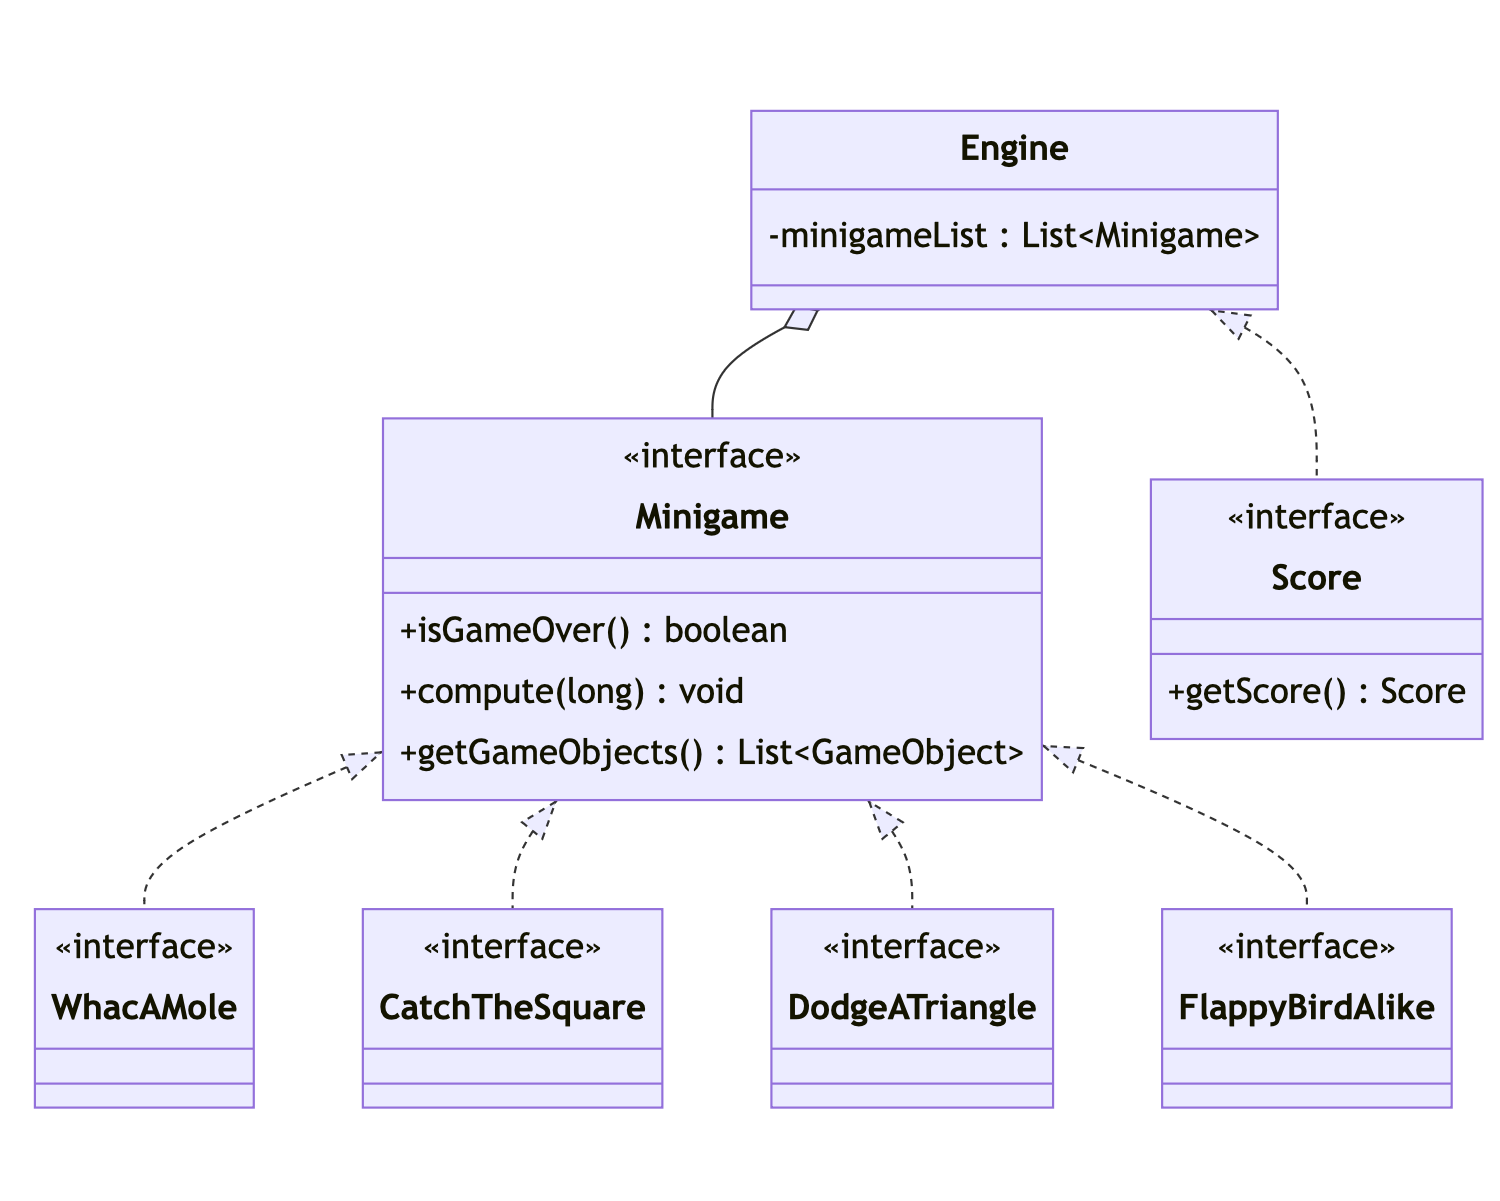
\includegraphics[width=\textwidth]{domain.png}
	\caption{UML diagram of the domain analysis}
\end{figure}

\chapter{Design}

\section{Architecture}
The project is built on the "model-view-controller" architecture: the \textbf{View} will be the entry point of the program.
At its creation it will instantiate the game window and the \textbf{Controller} class.
When the user decides to start the run it will be asked to the controller to create an \textbf{Engine}, this class will manage each \textbf{Minigame}.\\
The Model part is represented by the implementation of \textbf{Minigame}s these will contain \textbf{GameObject}s that will evolve over time with a specific logic.
The \textbf{Controller} directs the run with the game loop pattern, updating each frame the view with the \textbf{GameObject}s fetched from the \textbf{Engine}.
The \textbf{Controller} takes also care of intercepting the user's input from the \textbf{View}, then it forwards it to the Engine.
Once the input has been received, the Engine is responsible for communicating it to each minigame: these in turn will update the state of all the GameObjects they contain, i.e. every single entity in the various playing fields.

\section{Detailed design}
Each minigame is composed of \textbf{GameObject}s: those items use a component pattern, thanks to which we get
a full separation of concerns based on domains (allow a single entity to span multiple domains each other\footnote{From GPP, CH 14}).
\pagebreak
\begin{itemize}
	\item \textit{PhysicsModel}: Interface that deals with the physical state of a Game Object,
	      moving it according to its speed, considering the environment in which it is located (edges of the field)
	      and the other objects it interacts with (collision with obstacles).
	\item \textit{AspectModel}: It is the interface that orders the updating of the graphics of the single
	      object to the View, specifying which of the instructions already contained in SwingView need to be used.
	\item \textit{InputModel}: Interface related to a single GameObject that reads the input stored in the
	      engine and applies it, if the object recognizes it as its own command, changing its specifications (e.g. coordinates, speed).
	\item \textit{HitBoxModel}: Defines the shape and sizes of the hit box that the object shall interpret when colliding with other hit boxes.
\end{itemize}

\begin{figure}[ht]
	\centering{}
	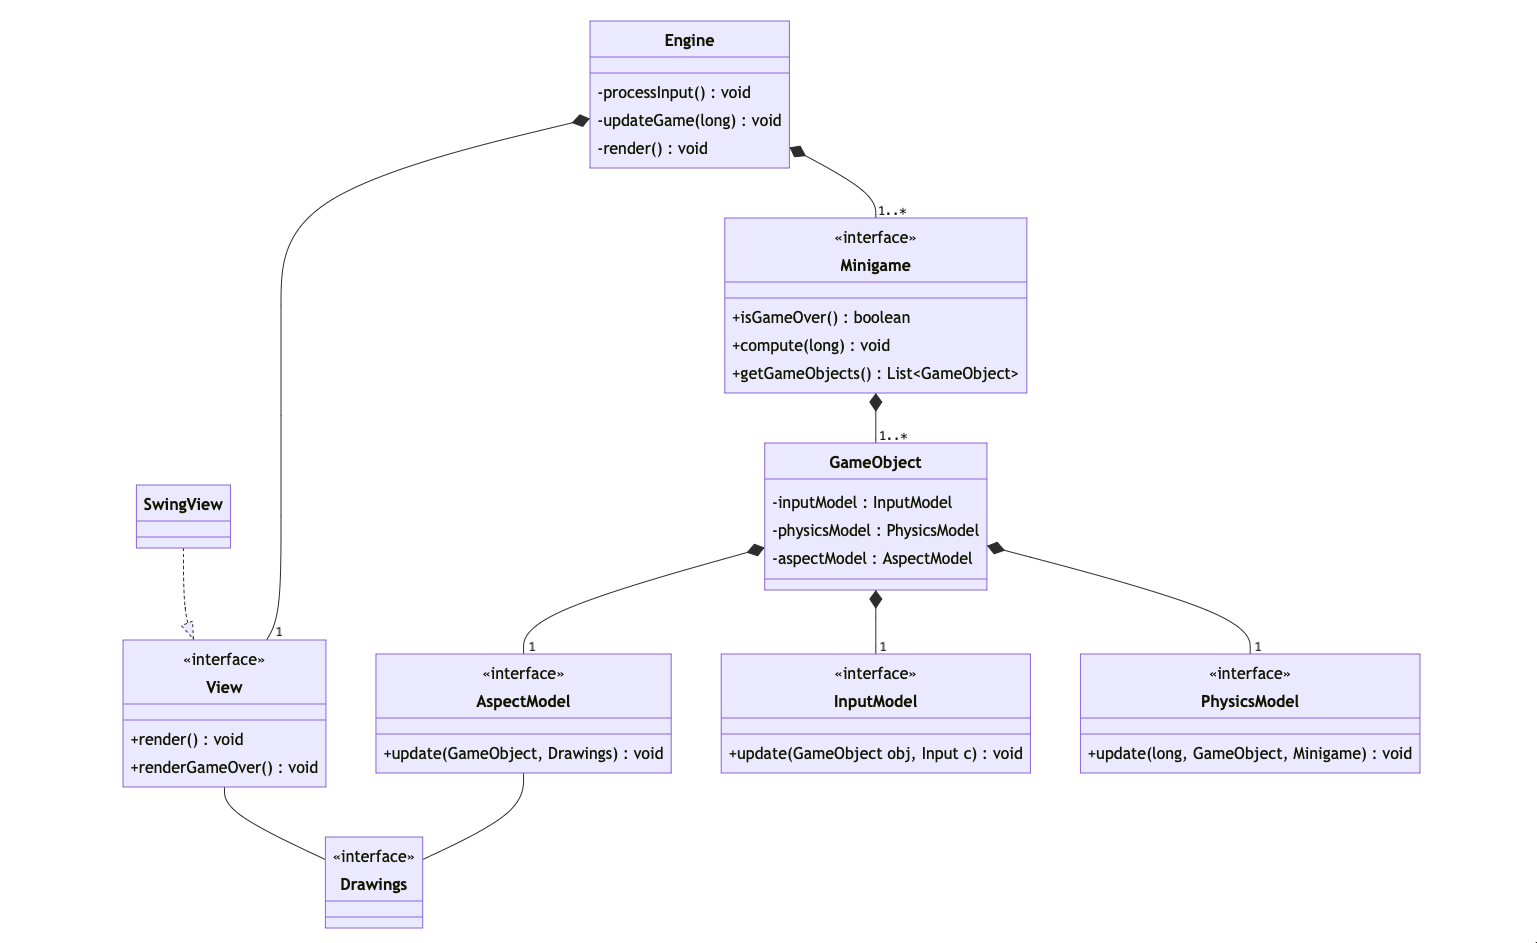
\includegraphics[width=\textwidth]{architecture.png}
	\caption{UML diagram of the architecture TODO MUST BE UPDATED}
\end{figure}
\subsection*{Leonardo Tassinari}
\textbf{Difficulty in CTS}\\
\textbf{Problem:} The spawn rate of the squares shall increase over time.\\
\textbf{Solution:} The CatchTheSquare's constructor adopts the strategy pattern taking a \textit{Function} interface. That function will return to the minigame the number of bombs that are expected to be spawn so far given the total amount of milliseconds elapsed from the beginning of the minigame.
My implementation of the function uses an exponential curve to increment the spawn rate progressively until a certain rate.
The limit rate is represented by the inclination of the line tangent to the exponential curve on the point where the derivate of the exponential reaches that steepness.\\
\begin{figure}[ht]
	\centering
	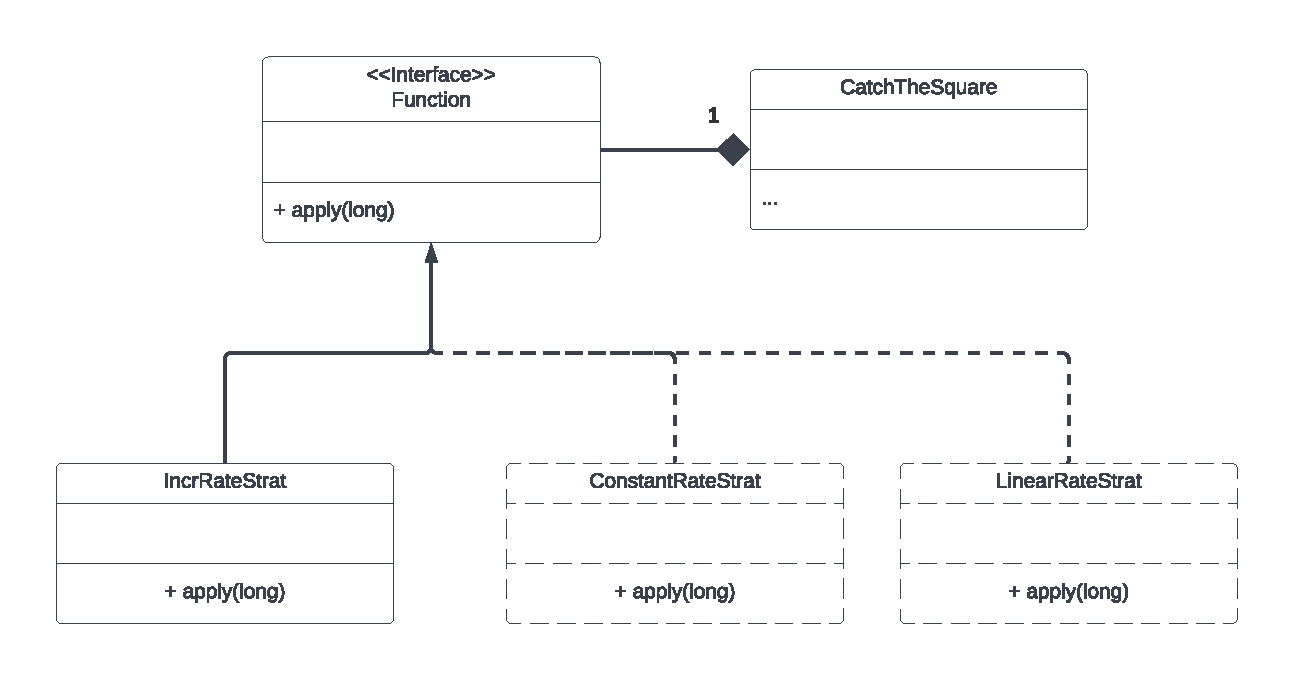
\includegraphics[width=\textwidth]{res/RateStrat.pdf}
	\caption{The corresponding UML diagram}
\end{figure}
\begin{figure}[ht]
	\centering
	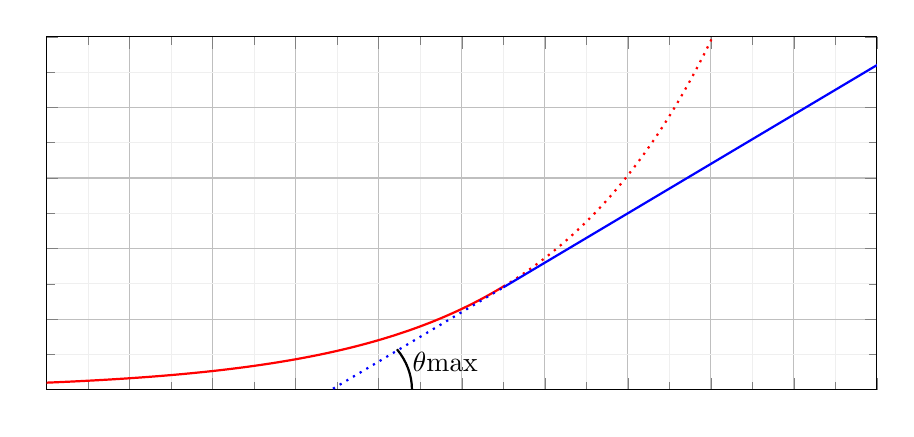
\begin{tikzpicture}
		\begin{axis}[
				xmin = 0, xmax = 100,
				ymin = 0, ymax = 50,
				xtick distance = 10,
				ytick distance = 10,
				xticklabels=\empty,
				yticklabels=\empty,
				grid = both,
				minor tick num = 1,
				major grid style = {lightgray},
				minor grid style = {lightgray!25},
				width = \textwidth,
				height = 0.5\textwidth
			]
			\addplot[
				domain = 0:55,
				samples = 200,
				smooth,
				thick,
				red,
			] {1.05^x};
			\addplot[
				domain = 55:150,
				samples = 200,
				dotted,
				thick,
				red,
			] {1.05^x};
			\addplot[
				domain = 55:150,
				samples = 200,
				smooth,
				thick,
				blue,
			] {x*0.7-24};
			\addplot[
				domain = 0:55,
				samples = 200,
				dotted,
				thick,
				blue,
			] {x*0.7-24};
			\pgfmathsetmacro{\angle}{asin(0.7/sqrt(1+0.7^2))} %asin(rise/hypotenus)
			\draw[black,thick] (axis cs: 44, 0) arc[start angle=0, end angle=\angle, radius=10];
			\node[black] at (axis cs: 48, 4) {\(\theta\)max};
		\end{axis}
	\end{tikzpicture}
	\caption{An example of the trend of the implemented function}
\end{figure}
\end{document}
